% Temporal DGNN Results Bar Chart
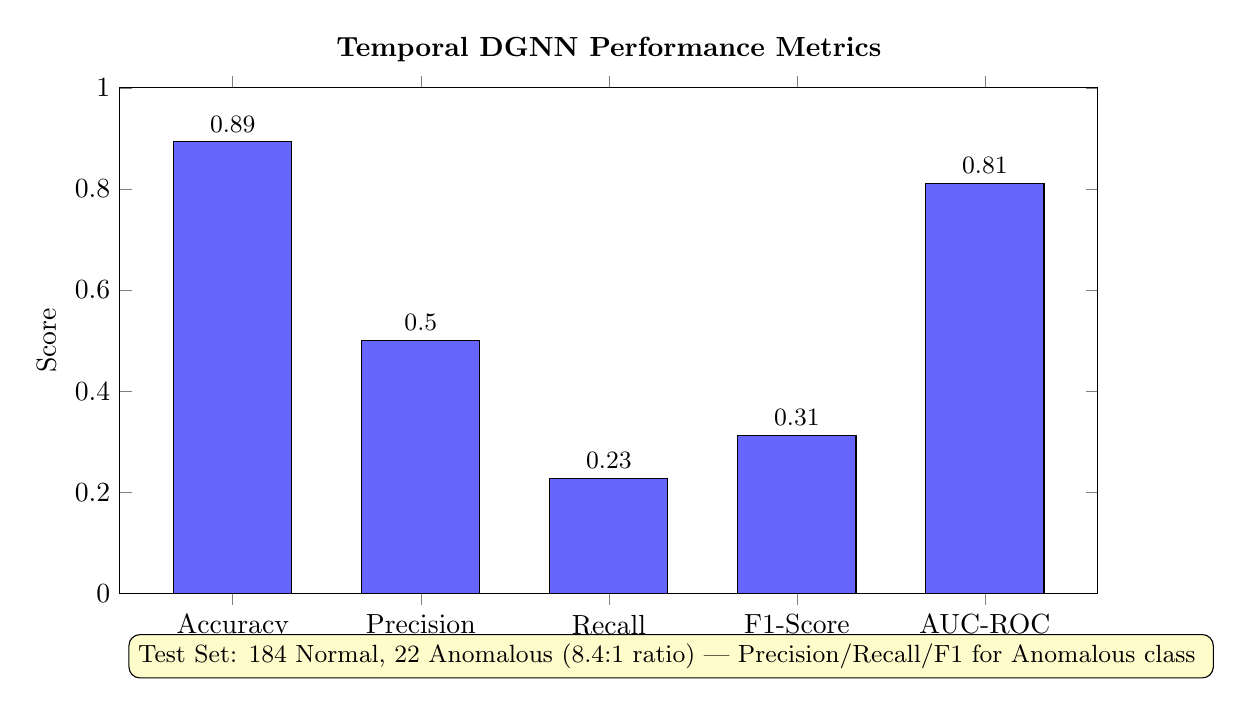
\begin{tikzpicture}
\begin{axis}[
    ybar,
    width=14cm,
    height=8cm,
    bar width=1.5cm,
    ylabel={Score},
    symbolic x coords={Accuracy, Precision, Recall, F1-Score, AUC-ROC},
    xtick=data,
    ymin=0, ymax=1,
    legend pos=north east,
    legend style={font=\small},
    title={\textbf{Temporal DGNN Performance Metrics}},
    title style={font=\bfseries},
    enlarge x limits=0.15,
    nodes near coords,
    nodes near coords style={font=\small},
]

% Metrics
\addplot[fill=blue!60] coordinates {
    (Accuracy, 0.8932)
    (Precision, 0.50)
    (Recall, 0.2273)
    (F1-Score, 0.3125)
    (AUC-ROC, 0.8116)
};

\end{axis}

% Notes
\node[font=\small, align=center, fill=yellow!20, draw, rounded corners] at (7, -0.8) {
    Test Set: 184 Normal, 22 Anomalous (8.4:1 ratio) | Precision/Recall/F1 for Anomalous class
};

\end{tikzpicture}
